%%%%%%%%%%%%%%%%%%%%%%%%%%%%%%%%%%%%%%%%%%%%%%%%%%%%%%%%%%%%%%%%%%%%%%%%
%%% AI Tutor: full system report, ECAI format
%%%%%%%%%%%%%%%%%%%%%%%%%%%%%%%%%%%%%%%%%%%%%%%%%%%%%%%%%%%%%%%%%%%%%%%%

\documentclass{ecai}

\usepackage{booktabs}
\usepackage{url}
\usepackage{tikz}
\usetikzlibrary{arrows.meta, positioning, shapes.geometric}

\begin{document}

\begin{frontmatter}

\paperid{1}

\title{AI Tutor: An Agentic Pipeline for Adaptive Learning}

\author[A]{\fnms{Bijesh}~\snm{P}}
\author[A]{\fnms{Hareesh}~\snm{Gowtham}\thanks{Corresponding Author. Email: hareeshgowtham90@gmail.com.}}
\author[A]{\fnms{Nagaraja}~\snm{S B}}
\author[A]{\fnms{Nagesh}~\snm{Poojary}}
\author[A]{\fnms{Navaneeth}~\snm{Kumar}}
\author[A]{\fnms{Sahana}~\snm{Gangasri}}
\author[A]{\fnms{Tejaswi}~\snm{Chitneedi}}

\address[A]{Indian Institute of Science, Bengaluru}

\begin{abstract}
AI Tutor turns an uploaded document into an interactive learning module. The
input can be a PDF, a slide deck, or a lecture transcript. A background
pipeline splits the document into topics. For each topic it writes an
explanation, a diagram, and comprehension questions. A separate adaptive tutor
is built as a LangGraph state machine. It asks the learner questions to gauge
their understanding. It tailors the explanation to that level and grades free
text answers. After a wrong answer it gives a hint or a simpler explanation.
The pipeline also produces a quiz, a mastery report, and a cohort analysis for
each module. This report describes the tutor architecture, the pipeline, and
three additions built on top of it. First, every language model call now passes
through a guardrail layer. The layer checks for prompt injection, output
safety, and topic relevance. It blocks a call with a clear message instead of
failing silently. Second, a knowledge graph is built for each module. It records
which concepts are prerequisites of others. The tutor can then ground a hint in
the right earlier concept rather than in text that only sounds similar. Third,
every generated question is tagged with one of six Bloom's taxonomy levels in
place of an informal difficulty label. We also report three reliability lessons.
Each recurred at a boundary between systems, and none came from the language
model's output itself.
\end{abstract}

\end{frontmatter}

\section{Introduction}

A static document is hard to learn from on its own. A good learning version
needs explanations at the right depth, diagrams, checks for understanding, and
a tutor that adapts to what the learner already knows. Building this by hand
does not scale. AI Tutor automates it with two systems that work together. A
content generation pipeline turns an uploaded document into a sequence of
topics. A short chain of language model calls then writes each topic's
explanation, diagram, and questions. An adaptive tutor runs a loop over those
topics. It diagnoses what the learner already knows, presents each concept at
the right depth, asks a follow up question, and then advances or remediates
based on the answer. The tutor also stores its hints and explanations in a
retrieval store built from the same content~\cite{lewis2020retrieval}.

The rest of this report is organized by section. Section 2 describes the
architecture. It covers the content pipeline, the adaptive tutor, and the tool
servers and vector store they both use. It also covers how the system reaches
different language model providers and how it evaluates its own output. Sections
3 to 5 describe three additions built on that architecture. Section 3 covers a
guardrail layer that checks every language model call for safety. Section 4
covers a knowledge graph that lets the tutor ground a hint in a prerequisite
concept rather than in similar sounding text. Section 5 covers the switch from
an informal difficulty label to Bloom's taxonomy levels. Section 6 reports three
reliability lessons that recurred at the boundaries of these systems. The
appendices give the supporting detail, and each one names the section it
supports.

\section{System architecture}

\subsection{Ingestion pipeline}

Before the content pipeline in Section 2.2 runs, a parser specific to the
file type turns it into one shared model of titled sections, so the rest of
the system never has to know which format a file started as. A PDF is read
through PyMuPDF, with each table of contents entry becoming one section, or
one section per page when no table of contents exists. A slide deck becomes
one section per slide. A Word file splits at each heading, folding the
paragraphs that follow into that section, or becomes one section when it has
no headings. A WebVTT transcript is split by its own classifier, covered in
Appendix A. Each parser also bounds how much of a file it reads, so a very
long document cannot push unbounded text downstream.

\subsection{Content pipeline}

A background thread splits an uploaded document into topics using a sliding
window over the text. After each chunk of accumulated text, a language model
call decides whether enough material has built up to form one coherent topic.
If no window closes cleanly before a length limit, the pipeline forces a
publish so the document still finishes processing. For each topic, a further
language model call writes an explanation. A separate call attempts a
diagram. The system checks that the diagram is well formed and has at least
one edge. If it is not, a second call writes a bullet point summary instead,
so every topic always ends up with a diagram or a summary. A further call
writes comprehension questions for the topic. Each topic is shown to the
learner as soon as its own chain finishes, rather than after the whole document
is done. The learner can start before later topics finish. Once every topic has
been processed, a final call writes the end of module quiz. The module is then
saved to the database and to the vector store described in Section 2.5.

\subsection{Adaptive tutor}

The adaptive tutor is a LangGraph state machine, shown in Figure 1. A
diagnostic call generates multiple choice questions on the learner's prior
knowledge of the upcoming topic. Scoring those questions is the only
deterministic step in the graph. It sets a presentation depth of beginner,
intermediate, or advanced. That depth then shapes the instructions for every
later call. Presenting a concept is itself a short chain of its own. If
the pipeline already enriched this topic, the tutor reuses that content and
adapts it to the learner's depth. If the topic was not enriched yet, the tutor
retrieves the closest matching content for that concept instead (Section 4).
This happens, for example, after resuming an unfinished session. The tutor then
asks a follow up question and grades the learner's free text answer with two
further calls. A correct answer moves on to the next concept. An incorrect
answer goes to a remediation step that either gives a grounded hint or
simplifies the explanation, then loops back to ask the question again.

\begin{figure}[t]
\centering
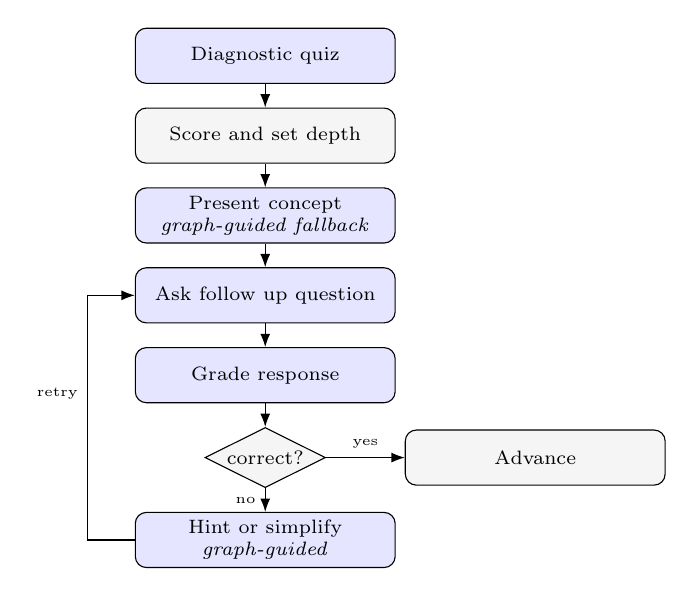
\begin{tikzpicture}[node distance=3mm and 3mm,
  every node/.style={font=\scriptsize},
  block/.style={rectangle, draw, rounded corners, align=center,
    minimum width=3.3cm, minimum height=0.7cm, fill=gray!8, inner sep=2pt},
  llm/.style={block, fill=blue!10},
  dec/.style={diamond, draw, align=center, inner sep=1pt, fill=gray!8, aspect=2},
  arrow/.style={-Latex}]

\node[llm] (diag) {Diagnostic quiz};
\node[block, below=of diag] (calib) {Score and set depth};
\node[llm, below=of calib] (present) {Present concept\\\textit{graph-guided fallback}};
\node[llm, below=of present] (ask) {Ask follow up question};
\node[llm, below=of ask] (eval) {Grade response};
\node[dec, below=of eval] (router) {correct?};
\node[block, right=10mm of router] (advance) {Advance};
\node[llm, below=of router] (remed) {Hint or simplify\\\textit{graph-guided}};

\draw[arrow] (diag) -- (calib);
\draw[arrow] (calib) -- (present);
\draw[arrow] (present) -- (ask);
\draw[arrow] (ask) -- (eval);
\draw[arrow] (eval) -- (router);
\draw[arrow] (router) -- node[above, font=\tiny]{yes} (advance);
\draw[arrow] (router) -- node[left, font=\tiny]{no} (remed);
\draw[arrow] (remed.west) -- ++(-0.6,0) |- node[pos=0.3, left, font=\tiny]{retry} (ask.west);

\end{tikzpicture}
\caption{The adaptive tutor. The score and set depth step and the correct
check are deterministic. Every other box is a language model call, and every
one of those calls now passes through the guardrail layer in Section 3. The
present concept, hint, and simplify steps use graph-guided retrieval
(Section 4) when a knowledge graph exists for the module.}
\label{fig:tutor}
\end{figure}

\subsection{Tool servers}

All effects outside the language model are isolated behind three tool
servers that follow the Model Context Protocol~\cite{anthropic2024mcp}, reached
through a single client. A document server parses an uploaded PDF, slide deck,
Word file, or transcript and extracts any embedded images. An assessment server
checks that a piece of generated output matches the shape the calling code
expects. A storage server saves a finished module to the database and reads
and writes the vector store in Section 2.5. Because every server is reached
through the same client, the pipeline and the tutor never import a parsing
library, a database driver, or the vector store's client directly. Appendix
A gives the full content pipeline diagram and the list of tools each server
exposes. It also covers the VTT transcript ingestion path. That path skips the
pipeline's own segmentation call, because a transcript already arrives split
into sections.

\subsection{Vector retrieval}

Right after a topic is enriched, its full explanation is embedded and saved
into a per module collection in a vector database, through the storage server.
A small embedding model runs locally for this~\cite{reimers2019sentence},
rather than through a separate provider call. This vector store is the system of
record for the actual text of each concept. The knowledge graph in Section 4 decides which concept's text is
worth fetching, but the text itself always comes from this store, never from
the graph. The tutor's hint and concept presentation calls query this store
only when the pipeline's own content for the current topic is missing. Every
query is filtered to the current module's identifier, for the reason given as
the third reliability lesson in Section 6.

\subsection{Multi-provider access}

An LLM factory gives the same uniformity on the model side that the tool
servers give on the data side. Every call site in this report is written
against one interface. A setting stored per user chooses whether calls go to
Anthropic, to Portkey, or to a local Ollama model. That setting can be changed
from the sidebar while the app is running. The full path from upload to a
finished tutor session has been checked end to end against all three providers.
Switching a deployment's model therefore changes only configuration, not the
pipeline or the tutor code.

\subsection{Evaluation and observability}

The system separates two kinds of evaluation that should not be mixed
together. The first judges the learner during a session and drives the
tutor itself. A language model call grades the learner's free text answer
and decides whether the concept is mastered, and a deterministic step scores
the diagnostic quiz and sets the presentation depth. The second judges the
tutor's own output quality after a session ends and does not affect the
session itself. Three metrics from DeepEval judge this output, each with a pass
threshold of 0.5. They score whether the tutor's answers were relevant to the
question asked, whether they stayed faithful to the source material, and
whether the explanation was clear. These metrics run only when a user presses a
Run Evals button on the observability page, so their cost stays under the
user's control rather than being automatic. The same provider already selected
for the session acts as the judge, so no separate key is needed. Every language
model call in the system also sends a trace to a local tracing server. A
developer can then inspect the calls a session actually made. Appendix F gives
the full table of which tutor steps drive mastery and the definitions of the
three quality metrics.

\section{Guardrails on every language model call}

The system makes its language model calls from fourteen call sites across
the tutor and the content pipeline. None of them had any check on what went in
or what came out. Two places carry text the system did not write itself into a
prompt: text extracted from an uploaded document, and the learner's own free
text answer in the tutor.

Every call now goes through a wrapper class. The LLM factory puts this wrapper
around the real provider client before handing it back to any caller. Because
the wrapper sits at the factory, every call site is covered without any change
to its own code. This includes call sites added later, such as the knowledge
graph's relation extractor in Section 4. The wrapper runs four checks. A prompt
injection check~\cite{greshake2023not} and an output quality check use a fixed
set of patterns and no further language model call. A content safety check and
a topic relevance check each use a second language model call against the same
relevance check runs only when the caller passes the current topic. Of the four
tutor functions that could do this, only one puts the learner's own words into
its prompt: the function that grades a free text answer. The other three build
their prompts from text the system already generated. Passing the topic to
those three would only check the system's own well formed text against itself,
with no safety benefit. If any check fails, the wrapper raises an error with a
plain message. The existing error handling in the tutor and the pipeline then
shows that message to the user, with no new code.

The two checks that need a second language model call do not block a session
if that second call itself fails. A failed safety check should not be worse
than no safety check at all. The two pattern based checks never fail this way,
since matching a fixed pattern cannot raise an error. Twenty six tests cover
the wrapper. Appendix B gives the full table of checks and a regression the
test suite caught while this layer was being built.

\section{Graph-guided retrieval}

Before this addition, the tutor had only one way to pull in outside material
for a hint or a fallback explanation: the plain similarity search in Section
2.4. That search has no notion that one concept is a prerequisite of another,
or that two concepts are related beyond sounding alike. This limited what a
hint could say. The tutor could re-explain the same concept the learner had
just gotten wrong, but it could not pull in the earlier concept the learner was
actually missing.

The system now builds a graph for each module~\cite{hogan2021knowledge}. The
graph records typed relationships between concepts, such as one concept being a
prerequisite of another, or two concepts being related. It is built once the
pipeline has
enriched every topic, since deciding how concepts relate needs the whole set of
concepts at once. A language model call reads a short list of the module's
concepts and returns the relationships it finds through a tool call. The system
drops any relationship that refers to a concept it does not recognize. If this
call fails for any reason, the module still gets a graph built from the parts
that need no language model, such as which topic follows which in the
document's own order.

When the tutor needs context, a retrieval function loads the module's graph
and picks concepts relevant to the current concept and the kind of help needed.
Presenting a concept pulls in related concepts and direct prerequisites. Giving
a hint pulls in prerequisites first, since a wrong answer often means a missing
earlier concept. Simplifying a concept pulls in prerequisites further back,
ordered from earliest to latest. The function then fetches each selected
concept's full text from the vector store in Section 2.5, the same store the
plain similarity search already used. The system falls back to that same plain
similarity search if a module has no graph yet, the current concept is not
known, or any step raises an error. This follows the same discipline as the
third reliability lesson in Section 6. Appendix C gives the full table of
relationship types and the retrieval algorithm.

\section{Bloom's taxonomy for question generation}

The system generates questions in four places: the end of module quiz, the
comprehension questions attached to each topic, the pre lesson diagnostic, and
the tutor's own follow up question. Each question used to carry an informal
label of easy, medium, or hard, with no real definition behind it. The system
now tags every question with one of Bloom's six cognitive levels
instead~\cite{anderson2001taxonomy}: remember, understand, apply, analyze,
evaluate, and create. This follows the prompting approach from Scaria et
al.~\cite{scaria2024bloom}. They tested
several ways to prompt a language model for a target skill level. They found
that three things worked best: giving the model a persona, asking it to reason
through the question before writing it, and stating each level's definition in
the prompt. Adding hand written example questions for each level made results
worse, so the system does not use examples here.

Each of the four places that generate questions uses a different slice of the
six levels, since each one serves a different purpose. The end of module quiz
mixes questions from all six levels in every attempt. The comprehension
questions use only the first three levels, since a quick check during reading
does not need the higher ones. The pre lesson diagnostic uses only remember and
understand, since it runs before the learner has seen any material. The tutor's
follow up question maps the learner's current presentation depth to a pair of
levels. This ranges from remember or understand for a beginner up to evaluate
or create for an advanced learner. Appendix D gives the full definitions of all
six levels and the question fields that changed to carry the new label.

\section{Reliability lessons}

Three problems recurred across both the pipeline and the tutor.

The first is a one time setup cost left on the path the learner waits on. The
vector store's embedding model downloads on first use, and the storage tool
server's first call pays a variable cost importing native libraries. Both
blocked the first content a new user saw, with no progress indicator and no
time limit. The fix was the same in both cases: pay the cost once at startup, in
a background thread, before any user reaches that code path, and give every call
across a process boundary an explicit time limit.

The second is that error handling does not cross from one runtime into
another. The diagram renderer runs in the learner's browser, after the Python
code that produced the diagram has returned and left its error handling behind.
A raw failure in the browser was therefore invisible to the server and reached
the learner directly. The fix was to catch the failure in the browser's own
code, check that the diagram is visible and well formed before measuring it,
give every render a time limit, and fall back to the bullet point summary from
Section 2.2.

The third is that retrieval should be a narrow fallback, not something run on
every call. An earlier version searched the vector store on every call and
sometimes returned text that read well but came from the wrong module, which
was worse than not searching at all. The tutor now searches only when the
pipeline's own content for a topic is missing, and every search is filtered to
the current module. Appendix E gives the full account of all three problems.



\section{Conclusion}

AI Tutor's content pipeline and its adaptive tutor are each a short chain of
language model calls. Retries, fallbacks, and a per call decision about whether
to ground the call in retrieved content connect that chain. Neither system is a
single prompt, and neither is a fully autonomous agent making its own plans.
The three additions in this report, the guardrail layer, the knowledge graph,
and the Bloom's taxonomy labels, were each added at the boundary of this chain
rather than by changing the chain itself. That is also why each one could be
tested and verified on its own. The reliability lessons in Section 6 point the
same way. Every recurring failure sat at a boundary: between two processes,
between two programming languages, or between a call site and the decision of
whether to retrieve for it. None sat inside the language model call itself.

\clearpage

\appendix {Appendix}

\section{Full architecture diagram (supports Section 2)}

Figure 2 gives the content pipeline in full, including the just in time
delivery loop and the final quiz generation step that runs once every topic
has published.

\begin{figure}[h]
\centering
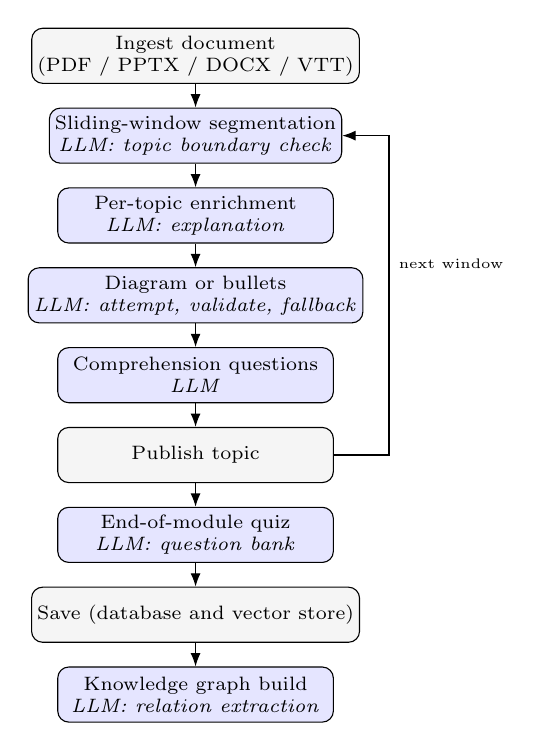
\begin{tikzpicture}[node distance=3mm and 3mm,
  every node/.style={font=\scriptsize},
  block/.style={rectangle, draw, rounded corners, align=center,
    minimum width=3.5cm, minimum height=0.7cm, fill=gray!8, inner sep=2pt},
  llm/.style={block, fill=blue!10},
  arrow/.style={-Latex}]

\node[block] (ingest) {Ingest document\\(PDF / PPTX / DOCX / VTT)};
\node[llm, below=of ingest] (segment) {Sliding-window segmentation\\\textit{LLM: topic boundary check}};
\node[llm, below=of segment] (enrich) {Per-topic enrichment\\\textit{LLM: explanation}};
\node[llm, below=of enrich] (diagram) {Diagram or bullets\\\textit{LLM: attempt, validate, fallback}};
\node[llm, below=of diagram] (questions) {Comprehension questions\\\textit{LLM}};
\node[block, below=of questions] (publish) {Publish topic};
\node[llm, below=of publish] (quiz) {End-of-module quiz\\\textit{LLM: question bank}};
\node[block, below=of quiz] (store) {Save (database and vector store)};
\node[llm, below=of store] (graph) {Knowledge graph build\\\textit{LLM: relation extraction}};

\draw[arrow] (ingest) -- (segment);
\draw[arrow] (segment) -- (enrich);
\draw[arrow] (enrich) -- (diagram);
\draw[arrow] (diagram) -- (questions);
\draw[arrow] (questions) -- (publish);
\draw[arrow] (publish.east) -- ++(0.7,0) |- node[pos=0.3, right, font=\tiny]{next window} (segment.east);
\draw[arrow] (publish) -- (quiz);
\draw[arrow] (quiz) -- (store);
\draw[arrow] (store) -- (graph);

\end{tikzpicture}
\caption{The content pipeline, with the knowledge graph build (Section 4)
added as a final step once every topic has been saved.}
\label{fig:pipeline}
\end{figure}

For a WebVTT transcript, the parser classifies each caption as teaching
content, a question and answer exchange, or non content chatter such as a
greeting or a scheduling remark, and discards the chatter. It removes speaker
identity entirely, so a section title names the topic or concept covered rather
than the person who said it. Speaker turns are still used internally, to find
where a question and answer exchange starts and ends. Because a transcript
already arrives broken into these sections, the pipeline's own segmentation
call in Section 2.2 is skipped for this input type. The same per topic
enrichment chain then runs directly on the parser's sections.

\begin{table}[h]
\caption{Tools exposed by each of the three servers.}
\label{tab:mcp-tools}
\centering
\small
\begin{tabular}{p{1.6cm}p{4.6cm}}
\toprule
\textbf{Server} & \textbf{Tools} \\
\midrule
Document & Parse a PDF, a slide deck, a Word file, or a transcript. Extract embedded images. \\
Assessment & Check that generated output matches an expected schema. \\
Storage & Save a module to the database. Add a topic's text to the vector store. Search the vector store. \\
\bottomrule
\end{tabular}
\end{table}

The vector store is a ChromaDB collection scoped to one module. A small model
produces the text embedded into it, running locally through the ONNX runtime
rather than a separate machine learning framework. This is why the first
reliability lesson in Section 6 describes a one time download cost rather than a
per call network cost. Each stored entry carries the module identifier and the
topic identifier as metadata. That metadata is what lets a query in Section 2.5
filter to the current module.

\section{Guardrail checks in full (supports Section 3)}

\begin{table}[h]
\caption{The four guardrail checks.}
\label{tab:guardrails}
\centering
\small
\begin{tabular}{p{1.6cm}p{1.0cm}p{1.6cm}p{1.0cm}}
\toprule
\textbf{Check} & \textbf{Side} & \textbf{Method} & \textbf{Always on} \\
\midrule
Prompt injection & Input & Fixed patterns & Yes \\
Topic relevance & Input & Second LLM call & Only with topic \\
Output quality & Output & Fixed patterns & Yes \\
Content safety & Output & Second LLM call & Yes \\
\bottomrule
\end{tabular}
\end{table}

The regression mentioned in Section 3 happened as follows. The function that
grades a learner's answer was changed to pass the current topic into the
shared \texttt{generate} call, so the topic relevance check could run. A test
that builds a provider client directly, without going through the guardrail
wrapper, then failed with an error. The shared interface that every provider
client implements did not yet declare a topic argument; only the wrapper did.
The fix added that argument, with a default of no value, to the shared
interface and to every provider client. A provider client used on its own and a
provider client wrapped in guardrails now accept the same call. The test suite
caught this before the change was committed. The lesson matches Section 6. A
change that looks safe because it only adds an argument can still break a caller
that does not go through the new code path.

\section{Knowledge graph detail (supports Section 4)}

\begin{table}[h]
\caption{Relationship types stored in the graph.}
\label{tab:kg-edges}
\centering
\small
\begin{tabular}{p{2.0cm}p{2.7cm}p{1.0cm}}
\toprule
\textbf{Relationship} & \textbf{Meaning} & \textbf{Source} \\
\midrule
Part of & Concept belongs to the module & Pipeline \\
Follows & Concept comes after another in document order & Pipeline \\
Prerequisite of & Learn the first before the second & LLM \\
Related to & The two concepts are closely linked & LLM \\
Elaborates & One concept is a deeper view of another & LLM \\
Mentions & Concept refers to a named term & Pipeline and LLM \\
Defines & Concept is the canonical definition of a term & LLM \\
\bottomrule
\end{tabular}
\end{table}

The graph is stored as a directed graph that allows more than one relationship
between the same pair of concepts. It uses the NetworkX
library~\cite{hagberg2008exploring} and is written to a file per module in the
GraphML format. GraphML keeps the typed attributes on each relationship and can
be opened and read in a text editor for debugging.
A relationship of the prerequisite type must not form a cycle, since a cycle
would mean a concept is a prerequisite of itself once you follow the chain
around. After extraction, the system checks for cycles. It removes the lowest
confidence relationship in any cycle it finds, then records that it did so.

The retrieval function takes the module, the current concept if known, a
plain text query to fall back on, and which of the three kinds of help is
needed. It loads the module's graph. If none exists, it calls the same plain
similarity search the tutor always had and returns that result directly.
Otherwise it selects candidate concepts as described in Section 4 and fetches
each one's full text from the vector store. If the graph returned fewer
concepts than the function was asked for, it tops up the remainder with plain
similarity search on the original query. The selected text is then joined
together and returned in the same shape the tutor's calling code already
expected. The calling code therefore needed only a small change to use this
function in place of the plain search it called before.

\section{Bloom's taxonomy levels in full (supports Section 5)}

The six levels run from lowest to highest. Remember is recalling a fact or a
definition. Understand is explaining an idea in your own words. Apply is using a
concept in a new situation. Analyze is breaking a concept into its parts and
seeing how they relate. Evaluate is judging a concept against a standard. Create
is putting parts together into something new. The field that used to hold a
difficulty label on a question now holds one of these six level names. A quiz
that used to be generated at a single difficulty is now generated as a mix
across all six levels in one pass.

\section{Reliability lessons in full (supports Section 6)}

The vector store's default embedding function downloads an eighty megabyte
model the first time it runs. Before the fix, this download happened on the
exact request that was building a new user's first topic. The user saw nothing
beyond a normal wait. The storage tool server has the same kind of cost on its
own first call. Importing the numeric libraries it depends on can take anywhere
from about one second to over thirty seconds, depending on what else is running
on the machine. A call with no time limit would simply hang if that import took
unusually long. Both costs are now paid once, in a background thread, when the
application process starts, well before any real user reaches that code path.
The storage tool server's client now also enforces an explicit time limit on
every call as a second line of defense.

The diagram rendering failure had three distinct causes, found one after
another. First, a diagram with no usable content still produced a non empty
string. The code that prepares the diagram's source text always adds a required
header line, even to an empty diagram, so a check for an empty string did not
catch this case and the renderer attempted to draw nothing. Second, a page that
shows several topics as tabs keeps every tab's content in the page at once and
only hides the ones not currently selected. The library that measures text size
for layout returns a size of zero for anything inside a hidden tab, and the
rendering library only measures text once. A diagram first rendered while its
tab was hidden therefore stayed broken even after the tab was opened. Third, a
diagram with a cycle in it could make the rendering library's layout step run
for an unbounded amount of time with no result. Each of these three was fixed
the same way: a check before depending on the thing that check verifies, a
visibility check before measuring, and a time limit on the layout step that
falls back to the same bullet point summary if the limit is reached.

The retrieval scoping problem showed up as the tutor occasionally giving a
hint that read fine on its own but was clearly about a different topic than the
one the learner was struggling with. Retrieval calls were then changed to
filter by the current module and to run only when the pipeline's own content
for the current topic was missing. This stopped happening, because the search
space for any one call became much smaller and only ever contained content that
could plausibly be relevant.


\section{Evaluation detail in full (supports Section 2.7)}

\begin{table}[h]
\caption{Steps that drive mastery during a session.}
\label{tab:eval-nodes}
\centering
\small
\begin{tabular}{p{1.8cm}p{0.5cm}p{2.9cm}}
\toprule
\textbf{Step} & \textbf{LLM} & \textbf{What it sets} \\
\midrule
Diagnostic quiz & Yes & The pre lesson questions \\
Score diagnostic & No & Presentation depth \\
Ask question & Yes & The follow up question \\
Grade response & Yes & Whether the concept is mastered \\
Give hint & Yes & Adds the hint to the chat history \\
Simplify & Yes & Resets the attempt count \\
\bottomrule
\end{tabular}
\end{table}

The three end of session quality metrics are an answer relevancy score, a
faithfulness score, and a clarity score. The answer relevancy score checks that
the tutor's explanation actually addresses the question asked rather than
drifting off topic. The faithfulness score checks that the explanation does not
say something the source material does not support. The clarity score, defined
for this project, checks that the explanation is understandable on its own.
Each metric passes at a score of 0.5 or above. Scores from a session are stored
per metric and later read back as a mean, a pass rate, and a count, rather than
being overwritten by the last value seen. A session with several questions
therefore gets one aggregated result per metric, instead of losing all but the
final answer's score.

\section{Future work}

A few gaps follow directly from the system described above. First, audio
narration is currently generated for each topic only when that topic is about
to be shown, rather than ahead of time. Pre-generating it for every topic
during the pipeline run, with a way to invalidate the cache when a topic is
regenerated, would remove that wait from the live tutoring path entirely. This
is in the same spirit as the pre-warming fix in Section 6. Second, the
guardrail layer in Section 3 checks topic relevance at one call site, because
that is the one site that puts a learner's own words into a prompt. If a later
change threads learner-authored text into the hint or follow up question calls,
those sites should gain the same check. Third, the knowledge graph in Section 4
is scoped to one module by design. Extending it to a learner's history across
modules, while keeping the same per-module filtering discipline from Section 6,
could let the tutor connect a new concept to material the learner already
completed elsewhere. Fourth, the quality metrics in Section 2.7 have not yet
been checked against actual learning outcomes, such as a learner's quiz score
after a tutoring session. That comparison would show whether the metrics
measure what the project intends. Finally, the relation extractor in Section 4
makes one call per module regardless of how many concepts the module has. For a
very large module, it may be worth splitting that call into smaller batches and
checking whether this changes the quality of the relationships it finds.

\bibliography{report}

\end{document}
